\begin{tikzpicture}[overlay, remember picture]
    \node[anchor=north west, rotate=0, gray, font=\tiny, text width=\paperwidth] at (current page.south west)  [xshift=0, yshift=1.25cm] {
    [4] Adam Nahum et al., Quantum Entanglement Growth Under Random Unitary Dynamics, Physical Review X, 7.3 (2017s)
    };
\end{tikzpicture}

% Quantum Entanglement Growth Under Random Unitary Dynamics:
\vspace{-0.5cm}
\phantom{42} \vspace{-0.5cm}

\begin{figure}[h]
    \centering
    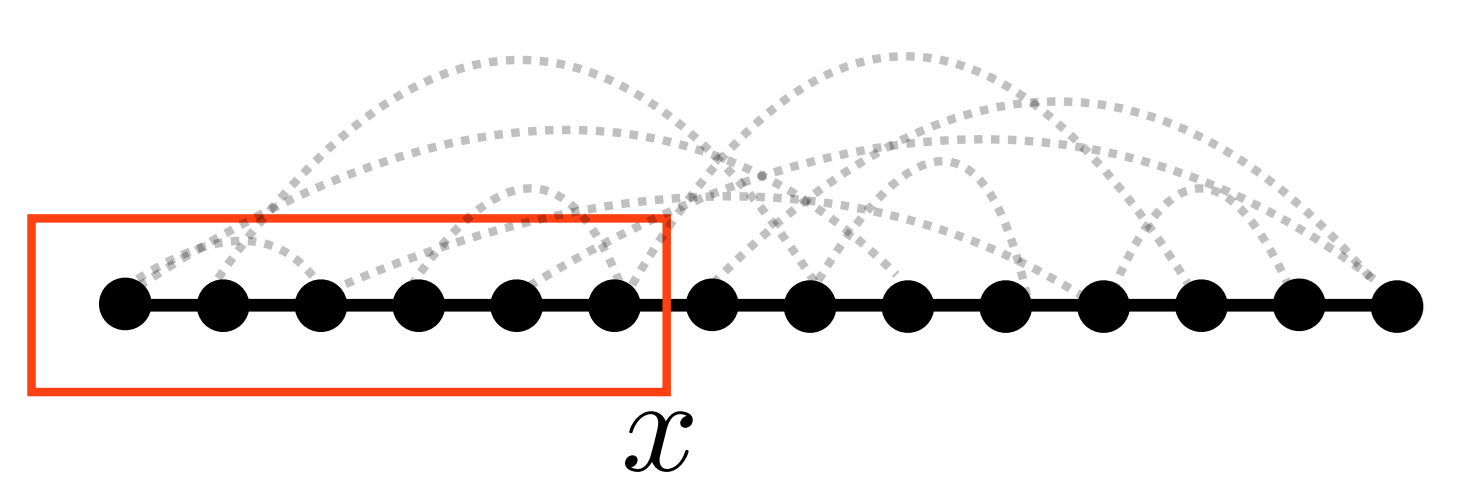
\includegraphics[width=0.4\textwidth]{imgs/guo_2.png}
    %\caption{}
    %\label{fig:}
\end{figure}

\vspace{-1cm}
Renyi entropy:
\begin{equation*}
	S_n(x) = \frac{1}{1-n} \ln(\tr \rho_x^n), 
	\hspace{5 mm} 
	|S(x+1) - S(x)| \leq 1.
\end{equation*}

With random updates \vspace{-4mm}
\begin{figure}[h]
    \centering
    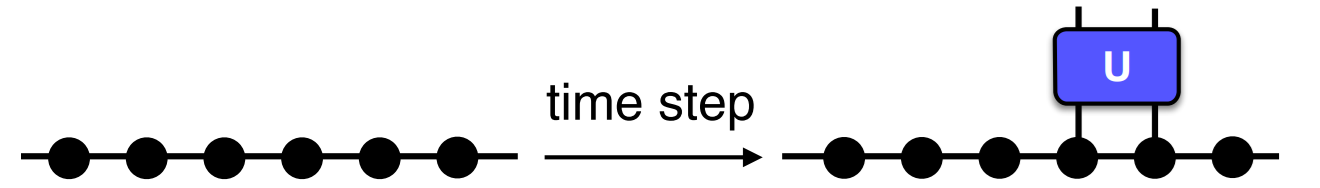
\includegraphics[width=0.5\textwidth]{imgs/guo_1.png}
    %\caption{}
    %\label{fig:}
\end{figure}

\vspace{-0.5cm}
\begin{equation*}
	S_0(x, t+1) = \min[S_0(x-1,t), S_0(x+1,t)] + 1
\end{equation*}

\vspace{-0.5cm}
\begin{figure}[h]
    \centering
    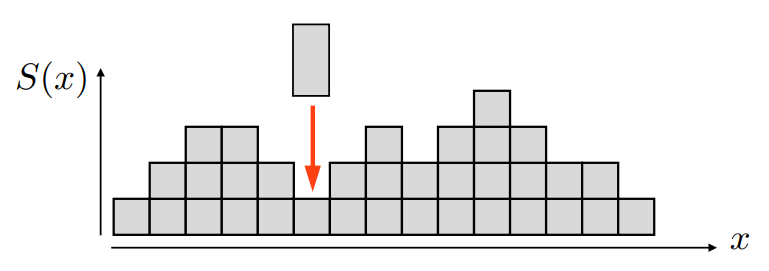
\includegraphics[width=0.5\textwidth]{imgs/guo_3.png}
    % \caption{}
    %\label{fig:}
\end{figure}
